\section{Observer}

The observer pattern is a software design pattern in which an object, called the subject, maintains a list of its dependents, called observers, and notifies them automatically of any state changes, usually by calling one of their methods. The observer pattern can cause memory leaks, known as the lapsed listener problem, because in basic implementation it requires both explicit registration and explicit deregistration, as in the dispose pattern, because the subject holds strong references to the observers, keeping them alive. This can be prevented by the subject holding weak references to the observers.

% Description of the design pattern
\subsection*{Example}

Figure~\ref{fig:Observer} presents the UML diagram of observer design pattern of project \textit{Follow}. In this diagram the \texttt{OutputDestination} interface is playing the role of observer and the class \texttt{FileFollowers} class is playing the role of subject for the observer design pattern.      

\begin{figure}[htb]
    \centering
    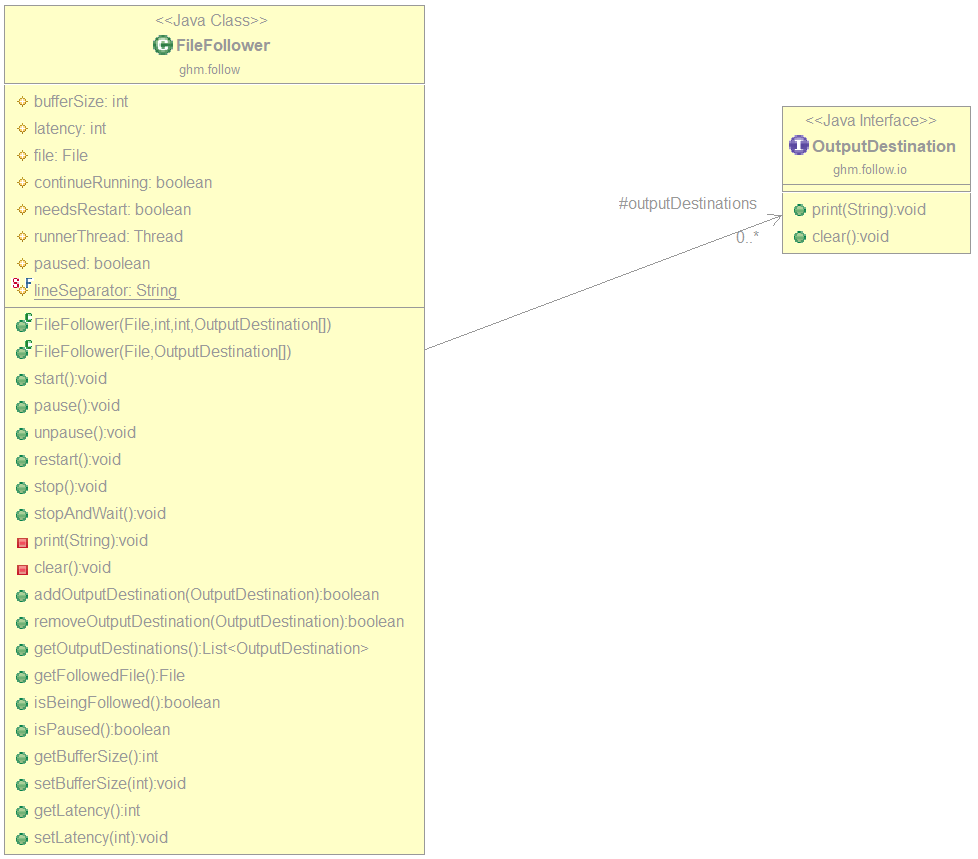
\includegraphics[width=\columnwidth]{images/Observer.png}
    \caption{Observer design pattern in the project \textit{Follow}}
    \label{fig:Observer}
\end{figure}
\FloatBarrier

% Description of the roles of the class in the design pattern

In Figure~\ref{fig:OutputDestination} observer interface has two methods \texttt{print} and \texttt{clear} and as you can see in the Figure~\ref{fig:FileFollower} and Figure~\ref{fig:Observer} the subject (i.e. \texttt{FileFollower}) has two common method with the observer that they can notify Observer about any changes, so that means \texttt{FileFollower} as subject for observer design pattern would not update itself directly and just call a method from \texttt{OutputDestination} interface as observer design pattern. 

%----------------------------------------------------------------------------------%
\begin{figure}[htb]
\centering
\lstset{language=Java, basicstyle=\scriptsize, stepnumber=1, showspaces=false, showstringspaces=false,breaklines=true}
\begin{lstlisting}

public class FileFollower {

	public FileFollower(File file, int bufferSize, int latency,
	        OutputDestination[] initialOutputDestinations) {
		this.file = file;
		this.bufferSize = bufferSize;
		this.latency = latency;

		int initOutputDestsSize = (initialOutputDestinations != null) ? initialOutputDestinations.length
		        : 0;
		outputDestinations = new ArrayList<OutputDestination>(initOutputDestsSize);
		for (int i = 0; i < initOutputDestsSize; i++) {
			outputDestinations.add(initialOutputDestinations[i]);
		}
	}


	public FileFollower(File file, OutputDestination[] initialOutputDestinations) {
		        initialOutputDestinations);
	}


	public synchronized void start() {
		if (continueRunning && paused) {
			unpause();
		}
		else {
			continueRunning = true;
			paused = false;
			runnerThread = new Thread(new Runner(), getFollowedFile().getName());
			runnerThread.start();
		}
	}

	public synchronized void pause() {
		paused = true;
	}

	public synchronized void unpause() {
		paused = false;
	}

	public synchronized void restart() {
		needsRestart = true;
		runnerThread.interrupt();
	} //Other method

\end{lstlisting}
\caption{[Observer] FileFollower.java}
\label{fig:FileFollower}
\end{figure}
\FloatBarrier

%------------------------------------------------------------------------------------%
\begin{figure}[htb]
\centering
\lstset{language=Java, basicstyle=\scriptsize, stepnumber=1, showspaces=false, showstringspaces=false,breaklines=true}
\begin{lstlisting}
public interface OutputDestination {
	public void print(String s);
	public void clear();
}
\end{lstlisting}
\caption{[Observer] OutputDestination.java}
\label{fig:OutputDestination}
\end{figure}
\FloatBarrier
%------------------------------------------------------------------------------------%



